\documentclass[a4paper, 10pt]{article}

\usepackage{times}
\usepackage[top = 1.2in, bottom = 1.2in, right = 1.2in, left = 1.2in]{geometry}
\usepackage[pdftex]{graphicx}
% \usepackage{setspace} %needed for
% \begin{onehalfspace}

\title{Real-time chat service for WunderBarKids}
\author{Pradnyesh Sawant}
\date{\today}    \vspace{-\baselineskip}
\pagestyle{empty}

\begin{document}

\maketitle
\thispagestyle{empty}   %maketitle has it's own pagestyle, so overwrite it with our own
% \tableofcontents

%\begin{abstract}
%\end{abstract}

% \begin{onehalfspace}

\section{Requirements}
Realtime chat cross browser, device and platform with video sharing service (Any language)

Time : 1 Week

\begin{itemize}
\item You are required to create a service to support realtime chat from multiple devices (browser, native clients, mobile etc)
\item User should be able to share videos
\item Client connectivity is going to be choppy hence service need to support sync methods
\item Design the platform (DB, Services, Interfaces) to support the above requirement
\item Design a simple REST api to aggregate a weekly information on who , what and when used this API
\end{itemize}

You should be able to answer the assumptions that you make for performance, extendibility and scalability.

\section{Introduction}
Even though I was required to create just the service, I created both the service and a web-based frontend, because of the following reasons:

\begin{itemize}
  \item Service would have been a ``pull'' model, and would have suffered from performance issues (see ``Performance Considerations -$>$ WebSockets'' section below)
  \item I was able to demonstrate my knowledge about the whole stack
\end{itemize}

\section{Service APIs}
\begin{tabular}[]{|l|l|p{2cm}|p{5cm}|p{2.1cm}|p{2cm}|}
  \hline
  URI & Type & Parameters & Sample Output & Functionality & Remarks \\ \hline
  /register & POST & email, passwd, passwd2, first-name, last-name & \{:status true :body "Registered sucessfully!"\} & Register user & \\ \hline
  /login & POST & email, passwd & \{:status true :body \{:id 2 :token ``pbkdf2+sha3-256\$5bd77a'' :name ``A B'' :users (\{:id 1, :first\_name "A", :last\_name "B", :email "a@b.com"\} \{:id 3, :first\_name "E", :last\_name "F", :email "e@f.com"\})\} & Login & \\ \hline
  /logout & POST & token & \{:status true :body "Logged-out successfully!"\} & Logout & \\ \hline
  /send-msg & POST & token, to, msg & -- & Send messages & Deleted, in favor of websockets (see below) \\ \hline
  /share & POST & token, to, vid & \{:status true :body \{:id 12, :from\_user\_id 1, :to\_user\_id 2, :message "", :datetime \#inst "2016-01-22T10:49:20.756-00:00", :file "resources/public/uploads/ring-multipart-5624539836408241247.mp4"\}\} & Share videos & \\ \hline
  /sync & GET & token, msg-id & \{:status true :body (\{:id 3, :from\_user\_id 1, :to\_user\_id 2, :message "ab -> cd", :datetime \#inst "2016-01-22T08:53:12.917-00:00", :file ""\} \{:id 6, :from\_user\_id 4, :to\_user\_id 1, :message "gh -> ab", :datetime \#inst "2016-01-22T08:53:42.729-00:00", :file ""\})\} & Sync messages & pass last-see-message-id \\ \hline
  /sync-vids & GET & token, msg-id & \{:status true :body (\{:id 11, :from\_user\_id 1, :to\_user\_id 2, :message "", :datetime \#inst "2016-01-22T08:58:07.690-00:00", :file "resources/public/uploads/ring-multipart-5624539836408241247.mp4"\} \{:id 12, :from\_user\_id 1, :to\_user\_id 2, :message "", :datetime \#inst "2016-01-22T10:49:20.756-00:00", :file "abc"\})\} & Sync videos & pass last-see-message-id \\ \hline
  /reports & GET & -- & \{:status true, :body (\{:id 1, :user\_id 1, :year 2016, :week 3, :num\_msg\_sent 5, :num\_msg\_recd 3, :num\_vid\_sent 1, :num\_vid\_recd 0\} \{:id 2, :user\_id 1, :year 2016, :week 3, :num\_msg\_sent 7, :num\_msg\_recd 1, :num\_vid\_sent 0, :num\_vid\_recd 1\} \{:id 3, :user\_id 1, :year 2016, :week 3, :num\_msg\_sent 2, :num\_msg\_recd 10, :num\_vid\_sent 1, :num\_vid\_recd 1\})\} & Weekly reports & NOTE: only till the last week, nothing for current week \\ \hline
\end{tabular}

\section{System Design}
In the real world scenario, the system design should look as shown below:

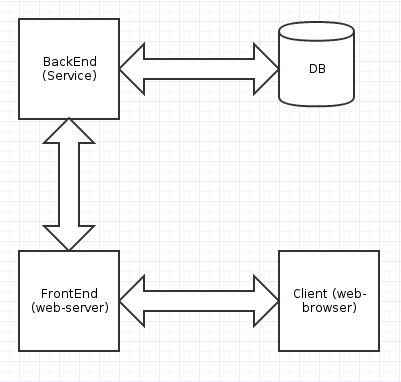
\includegraphics[width=6in]{ideal.png}

However, in our case, it looks like as shown below. This is because of the following reasons:

\begin{itemize}
  \item Due to security policies, JS can only talk to it's originating server =$>$ backend and frontend need to be separate servers
  \item It would have been an overkill (and too much effort) to create and maintain 2 servers (backend and frontend)
  \item So I ended up clubbing the 2 servers, but keeping the actual code modular such that it can be easily separated in the near future if need be
\end{itemize}

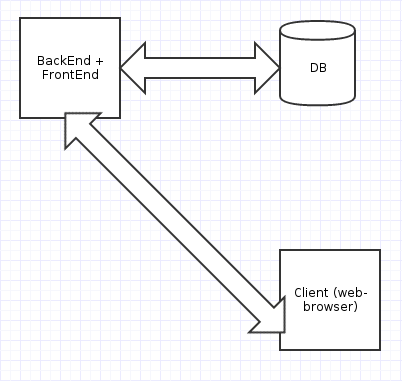
\includegraphics[width=6in]{implemented.png}

I have used the following stack:
\begin{itemize}
  \item DB: postgresql
  \item web-server: http-kit (http://www.http-kit.org/)
  \item programming language: clojure+clojurescript
  \item (notable) libraries used:
    \begin{itemize}
    \item luminus: initial project template
    \item selmer: html templating
    \item ring: server-side middleware
    \item bouncer: encryption
    \item buddy: validation
    \item cronj: cron-jobs
    \item bootstrap: css
    \item figwheel: rapid clojurescript development
    \item reagent: clojurescript wrapper to FaceBook react.js
    \item cljs-ajax: for AJAX
    \end{itemize}
\end{itemize}

\section{Performance Considerations}
\subsection{WebSockets}
In the initial design, I had a ``/send-msg'' POST API. However, while creating the frontend I realized that this is a extremely non-performant way of doing things, because it was necessary to call the ``/sync'' API multiple times every second to achieve the ``real-time'' effect. This would have, obviously, created exponetially more requests as the number of clients grew. And, even though the response body was pretty small (actually, empty, most of the time), the sheer number of requests to the server would have been too much.

The obvious solution was to use ``websockets'' and get rid of the ``send-msg'' API. The advantages of using this approach are:

\begin{itemize}
  \item The load on the servers (frontend -$>$ backend -$>$ database) reduces to less than 1\% of it's previous value
\end{itemize}

The disadvantage of using this method are:

\begin{itemize}
  \item File sharing cannot be done over websockets. So we need to create another pair of APIs (``/share'' and ``/sync-vids''). Also, to keep server load low (and have a non-realtime effect), we set the interval for calling the ``/sync-vids'' API to every 10 seconds
\end{itemize}

\subsection{Cron Jobs}
Cron jobs are needed for the following 2 tasks
\begin{itemize}
  \item Weekly report generation (not really a performance thing)
  \item Delete old (seen-by-user) messages and shared-files: this will reduce the DB size and disk usage and will thus improve performance
\end{itemize}
Both the jobs run on a weekly schedule

\section{Miscellaneous}
\subsection{State}
I have used ``atom'' (a clojure data-structure) to maintain in-memory state, like
\begin{itemize}
  \item last-seen-msgs for every user
  \item websocket channels
  \item etc...
\end{itemize}
These states need not be stored in DB; the worst thing that will happen if this state is lost is that the user will find himself logged-out from the system =$>$ a bad user-experience, but not a critical one for this assignment. It can be easily replaced with memcached or redis in a real-world application.

\subsection{Demo Videos}
You will also find the following demo videos, that demonstrate the running application, in the current folder

\begin{itemize}
  \item user-registration.mp4
  \item login.mp4
  \item real-time-chat.mp4
  \item sync-feature.mp4
  \item video-sharing.mp4
\end{itemize}

\subsection{Running The App}
To deploy and run the app on a local machine, please follow these steps (steps prepended with a \$ need to be executed at the terminal):

\begin{itemize}
  \item Install java (jdk)
  \item Install postgresql (and create database with following credentials)
    \begin{itemize}
    \item DB name: wbk\_dev
    \item DB username: wbk
    \item DB passwd: wbk
    \end{itemize}
  \item Install leiningen (http://leiningen.org/\#install)
  \item \$ git clone https://github.com/spradnyesh/wbk-chat-be
  \item \$ cd wbk-chat-be
  \item \$ lein migratus migrate
  \item Now in 2 different terminals run the following commands:
    \begin{itemize}
    \item \$ lein run
    \item \$ lein figwheel
    \end{itemize}
  \item visit location ``http://localhost:3000'' in the browser
\end{itemize}

\subsection{Open-Source Contribution}
During implemetation of this assignment, I was able to fix the issue regarding

http://www.luminusweb.net/docs/websockets.md\#adding\_the\_routes\_to\_the\_handler

(see ``***important***'' part). I will submit a pull-request for the same shortly.

% \end{onehalfspace}
\end{document}
